%-----------------------------------------------------------------------------------------------------------------------------------------
% PACKAGES
%Document Class starts every LaTeX document.  In this case, we're declaring the document class to be a book.  Changing "oneside" to "twoside" changes where the page numbers and headers and such get placed.
\documentclass[12pt,oneside]{book}

%These are the packages I used.  There's a description of (most of) them below (that Arthur wrote):
\usepackage{fancyhdr, geometry, graphicx, epstopdf, lscape, setspace, amssymb, amsmath, wasysym,moreverb, natbib, titlesec, longtable, multirow, alltt,here, indentfirst,ifthen}

\usepackage[small,bf]{caption}
\geometry{letterpaper}


%The "raggedbottom" command allows LaTeX to take some liberty with where the text on a page ends. This saved me some weird formatting problems I was having.
 \raggedbottom
 
%set the pagestyle:
\fancypagestyle{plain}{
\fancyhf{} % clear all header and footer fields, we will re-format them later

%Some formatting stuff:
\renewcommand{\headrulewidth}{0pt}
\renewcommand{\footrulewidth}{0pt}}
\newcommand{\nat}{Nature}

%	NECESSARY PACKAGES
%	fancyhdr enables use of fancy pagestyle
%	geometry defines page layout
%	graphicX allows for inclusion of graphics and page scaling and rotation
%	epstopdf allows the conversion of eps files to pdf and is required for figures
%	caption allows the captioning of figures
%	lscape allows for the creation of landscape pages-- important for large tables
%	setspace allows for doublespacing
%	natbib allows for the citations and Bibtex
%	titlesec allows for the definition of title layouts

%	OPTIONAL PACKAGES
%	aastex is only useful for article submission
%	revsymb is for physics symbols
%	amssymb is for math symbols
%	amsmath is for math formatting for things like matrices
%	parskip (\usepackage[parfill]{parskip})  allows paragraphs to begin with empty line
%	mathrsfs is required for \mathscr, the best Lagrangian and FT font
%	here makes !h force graph here and !t force the graph at the top of the page
%	wrapfig allows the wrapping of figures
%	fontspec allows the specification of fonts
%	color allows for the specification of the color of fonts
%	eso-pic allows the addition of watermarks such as a draft date


%-----------------------------------------------------------------------------------------------------------------------------------------
% RULES

%This has something to do with headers and margins and stuff:
\DeclareGraphicsRule{.tif}{png}{.png}{`convert #1 `dirname #1`/`basename #1 .tif`.png}
\textwidth 5.750in \textheight=8.50in \headheight 0.0625in \topmargin 0.0in % book strict

%==============================================================================
% Uncomment below for one sided printing (margins the same on even and odd pages)
\oddsidemargin 0.500in \evensidemargin 0.500in

% Uncomment below for two sided printing (margins different on even and odd pages)
%\oddsidemargin 0.563in \evensidemargin 0.2500in

%This sets how we want the formatting of chapter titles to look (bold face and Huge):
\titleformat{\chapter}{\bf\Huge}
{Chapter \thechapter}{-4.4em}{\\}
\titlespacing*{\chapter}{0pt}{-.57in}{*3}

%This formats the section headings:
\titleformat{\section}{\bf\Large}
{\thesection}{1em}{}
\titlespacing*{\section}{0pt}{*2}{*2}

%Let's double-space the document:
\doublespacing

%And our citation style will be aa (astronomy style):
\citestyle{aa}

%-----------------------------------------------------------------------------------------------------------------------------------------
% DOCUMENT/ TITLE PAGE
%Now the document actually begins:
\begin{document}

%This states that this is the stuff that comes before the real text:
\frontmatter

%Here goes the title page:
\pagestyle{empty}
\begin{titlepage}
\begin{center}
\rule{5.75in}{1pt} \\
\vspace*{-0.125in}
{\large \doublespacing Wesleyan University} \hfill {\large \doublespacing The Honors College}
\rule[0.2in]{5.75in}{1pt} \\
\vspace*{0.8in}
{\LARGE \singlespacing \bf Necroplanetology: \\ Dead Planets \\Are Fun} \\
\vspace*{0.05in}
\vspace*{0.10in}
{\large \vspace*{0.20in}  \singlespacing by \vspace*{.2in}
\\Girish Duvvuri \\ Class of 2017\\}
\vspace*{0.25in}
\vspace*{0.8in}
{\large \singlespacing A thesis submitted to the\\ faculty of Wesleyan University\\ in partial fulfillment of the requirements for the \\ Degree of Bachelor of Arts\\ with Departmental Honors in Astronomy\\ \vspace*{-0.15in} }
\vspace*{.25in}
\rule{5.75in}{1pt} \\
\vspace*{-0.125in}
{\large \doublespacing Middletown, Connecticut \hfill Eventually, 2048}
\rule[0.2in]{5.75in}{1pt} \\
\end{center}
\end{titlepage}


%-----------------------------------------------------------------------------------------------------------------------------------------
% ABSTRACT/ ACKNOWLEDGEMENTS
%After the title page, comes anything else you want before the Table of Contents.  Note that the Epigraph and acknowledgements are in their own files.  The \include command inserts the external files into the final document.

\pagestyle{empty}
%\pagestyle{plain}

\mbox{}
\vspace{.75in}
\hrule

\vspace{2in}


%\begin{minipage}[c]{4in}
\begin{centering}
	\hspace{.25in} 
	\parbox{5in}{
		\noindent 
		\textit{Well Shit.}
		\vspace{3pt}

		\begin{flushright}
			{\sc {--Varric Tethras}}\\
			{\textit{Dragon Age Inquisition}}
		\end{flushright}
	}
\end{centering}
\vspace{2.25in}
\hrule
\vfill



%\flushleft















\textwidth 5.750in \textheight=8.50in \headheight 0.0625in \topmargin 0.0in % book strict



\chapter*{Acknowledgements}



\titlespacing*{\chapter}{0pt}{*2}{*3}
Thank you D.S. (for sending) and H.R.S. (for making).

%My title formatting changes after the frontmatter, because of how i formatted my acknowledgements:

\titleformat{\chapter}{\bf\Huge}
{Chapter \thechapter}{-4.4em}{\\}
\titlespacing*{\chapter}{0pt}{*2}{*3}

\titleformat{\section}{\bf\Large}
{\thesection}{1em}{}
\titlespacing*{\section}{0pt}{*2}{*2}


%-----------------------------------------------------------------------------------------------------------------------------------------
% CONTENTS/ RULES OF HEADERS
%LaTeX creates a table of contents for you automatically, but you may have to compile the document twice before it shows up properly:

\tableofcontents  \pagestyle{empty}

%You can also put in the following, if you wish:

%\listoffigures
%\listoftables \pagestyle{empty}


%Now we start the real part of the document:
\mainmatter


%-----------------------------------------------------------------------------------------------------------------------------------------
% HEADERS
%This took me forever to figure out properly, and you may want to change it.  There's also different thing you can do if you want doublesided printing.  Your final thesis, as published by the University, is one-sided.


\renewcommand{\chaptermark}[1]{ \markboth{\sc\thechapter.\ #1}{}}

\pagestyle{fancy}
\fancyhead{}
\fancyfoot{}

\fancyhead[L]{\leftmark}
\fancyhead[R]{\thepage}

%==============================================================================
%Number your pages!  
\pagenumbering{arabic}

%-----------------------------------------------------------------------------------------------------------------------------------------
% CHAPTERS
%Here's the actual thesis:  (note that file names CAN'T have spaces in them!)

\chapter{Introduction}
\label{intro}

Background Info on white dwarfs and exoplanetary systems:
\section{Exoplanets}
Rise of the field, importance for understanding diversity of planetary systems
Context for pulsar planet as first exoplanet detection, lead in to post-stellar evolution objects. 

\textbf{Work notes:} mostly text, lit review.
\section{Transits}
Introduction to transit method (not very long)
Discussion of why WDs are favorable for transit detections: comparison figure of lightcurves for Earth transiting Sun vs WD

\textbf{Work notes:} mostly text, lit review. Make one figure.
\section{WD Transit Motivation}
Debris disks+ Polluted WDs: frequency, sinking timescales, overview of past work as motivation for transit studies. We know there are planetary remnants there.
K2 mission and guest proposals.

\textbf{Work notes:} Text. lit review +  go over other K2 guest proposals.
\section{WD1145 Detection}
Details regarding detection and a little information about followup photometry (more in Chapter \ref{chapter_photo}). 
Then \cite{Xu2016} detection of circumstellar absorption, leads into discussion of next section.

\textbf{Work notes:} Do some work with available K2 photometry papers to find the best way to summarize object's behavior. Pick out a stellar line to show CS absorption clearly: strong, isolated, preferably from Xu data to show blue and red edges. Or a more large-scale view like \cite{Xu2016} Fig 1a/b?
\section{Significance of WD1145} 
Explanation of lack of knowledge of planetary interiors: RV + transit constrain Mass/Radius $\implies \rho$, transit and eclispse spectroscopy give atmospheric info, but now we use WD as our mass spectrometer to get information about planetary interior. To give context, list some other known disintegrating planetary systems or other ways we've constrained composition (find the iron exo-Mercury that was identified because its orbital period requires that composition to avoid the disintegration we see here)

\textbf{Work notes:} lots of lit review (bring in work with disks, but not too much because that will get discussed more in Chapter \ref{chapter_spectra})


\section{Figure+Citation}

Look figure + citation: \citep[e.g.,][see Fig. \ref{PrettyPic}]{Vanderburg2015}. 

\begin{figure}
\centering
\scalebox{0.45}{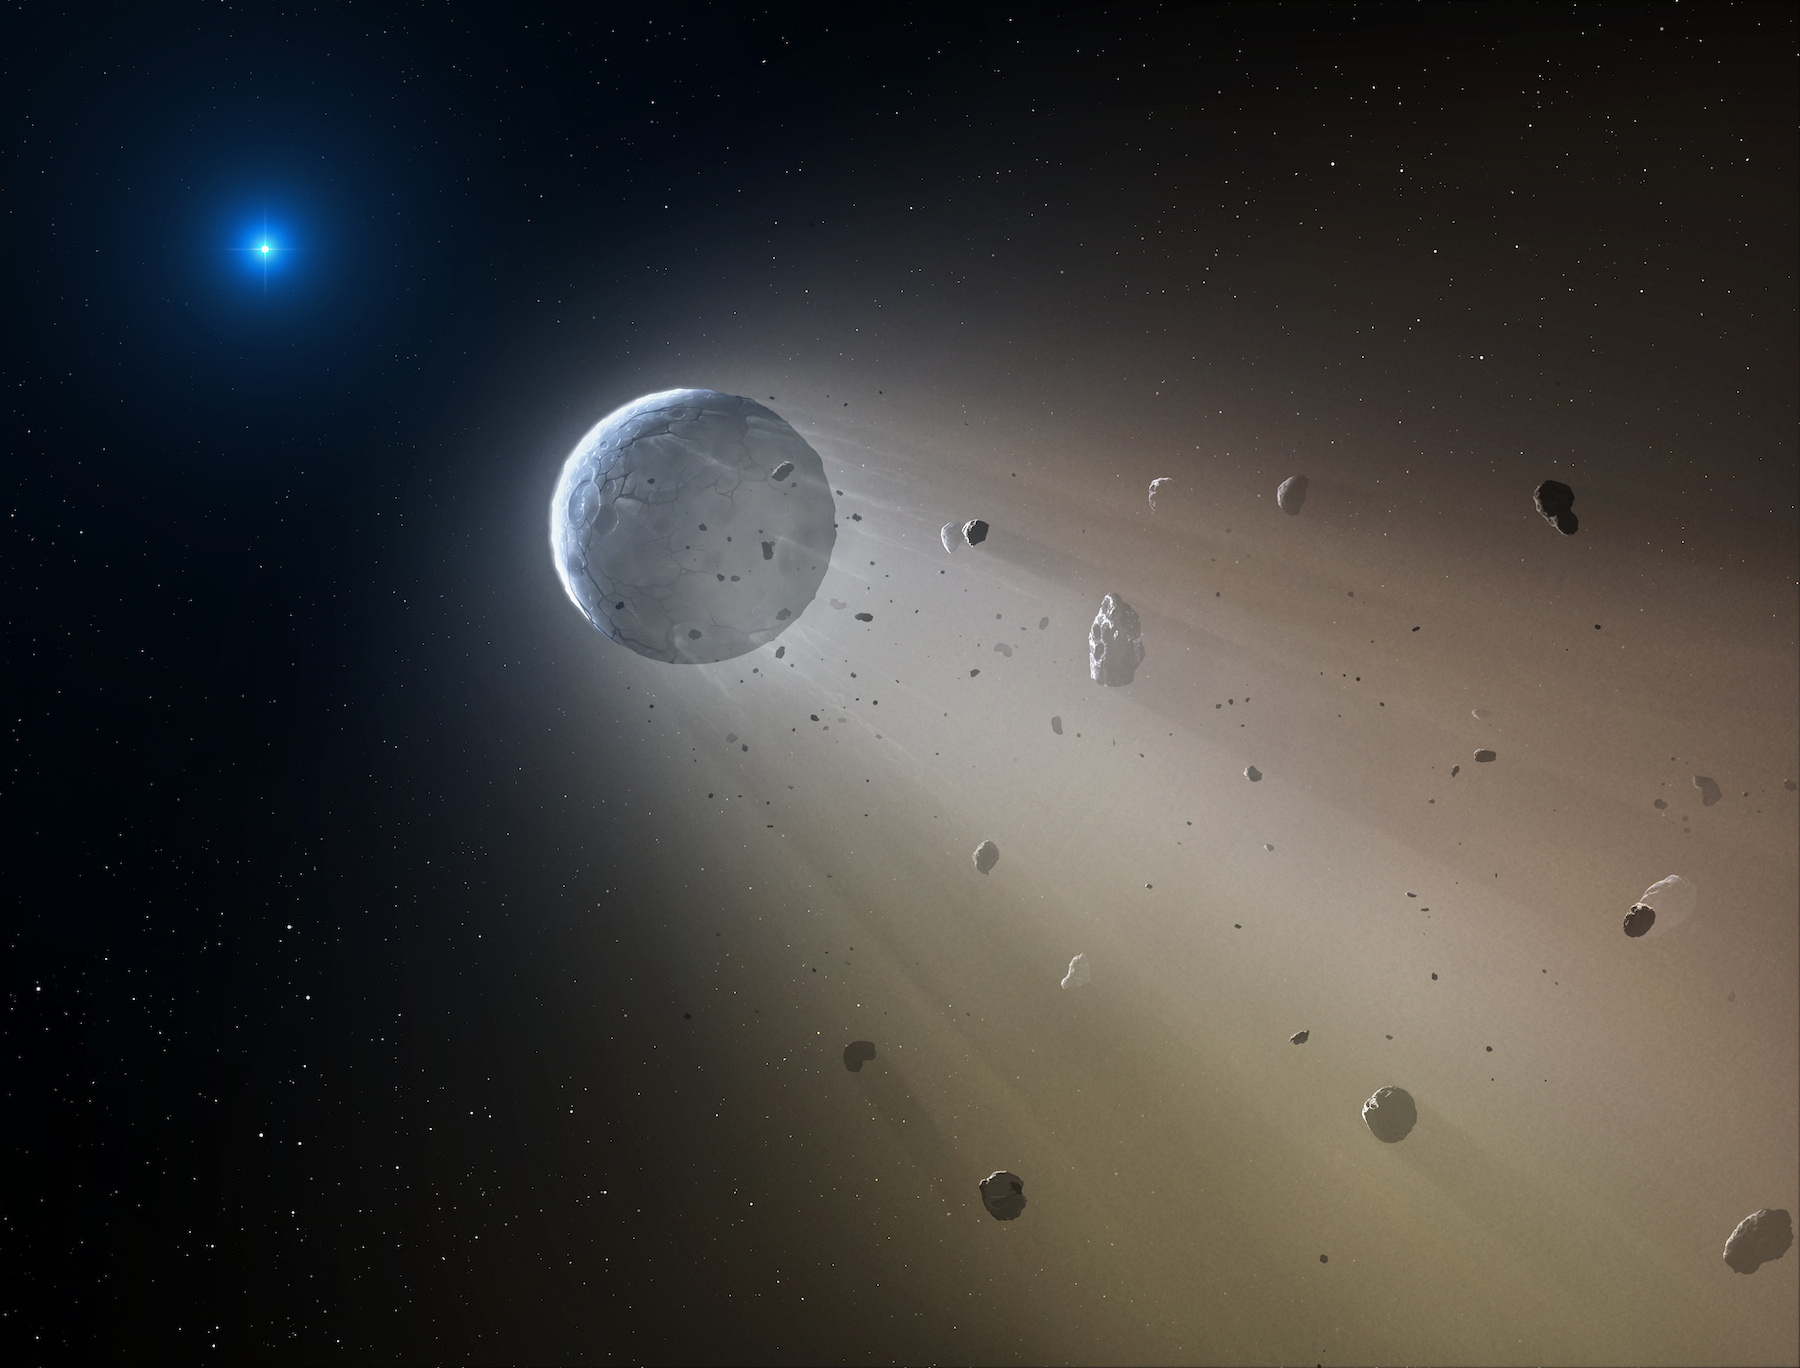
\includegraphics{Figures/PrettyPic.png}}
\caption{The artist rendition of WD1145+017 \citep[from][]{Vanderburg2015}.}
\label{PrettyPic}
\end{figure}

%\ifthenelse{\isodd{\thepage}}{\clearemptydoublepage}{}
\chapter{New Chapter is Easy}
\label{chap2}

Behold. 


\section{Sections are the Same}
\label{section2}
New sections are also easy.
	 
% \ifthenelse{\isodd{\thepage}}{\clearemptydoublepage}{}




%-----------------------------------------------------------------------------------------------------------------------------------------
%% APPENDIX

%tell LaTeX that you're now in the appendix section:

\appendix

%I wanted my title formatting to be slightly different here, so that things are numbered "Appendix A" instead of "Chapter A" or "Chapter 6"

\titleformat{\chapter}{\bf\huge}
{Appendix \thechapter}{-5.35em}{\\}
\titlespacing*{\chapter}{0pt}{-.5in}{*3}

%These are the file names of my appendices:


\chapter{Nonsense}
\label{appendix}
Appendices are TEXnically indistinguishable from normal chapters. 

\subsection*{Subsections are Possible?}

Apparently.





\doublespacing


%-----------------------------------------------------------------------------------------------------------------------------------------
%%BIBLIOGRAPHY:

\fancypagestyle{plain}{%
% clear all header and footer fields, we don't want these for the bibliography
\fancyhf{} 
% except we want the page number to show up in the center of the footer:
\fancyfoot[C]{\thepage} 

\renewcommand{\headrulewidth}{0pt}
\renewcommand{\footrulewidth}{0pt}}
\pagestyle{plain}

%change title spacing once again, for the bibliography:
\titlespacing*{\chapter}{0pt}{-.75in}{*3}

%Add the bibliography to the table of contents, it doesn't show up by default, you have to specify it:
\addcontentsline{toc}{chapter}{\textbf {Bibliography}}

%The default for BibTex (the bibliography builder in LaTeX) is to not include citations that are in your bibliography file, but that you don't cite anywhere in the paper.  This changes that setting, so that all papers show up in the bibliography, whether or not you referenced them:
\nocite{*}

%Insert the bibliography (in this case, my file name was also "bibliography" if not, your line would read: \bibliography{my_workscited_filename} or whatever:
\bibliographystyle{apj}
\bibliography{bibliography}

%the end!
\end{document} 